\documentclass[a4paper, 12pt]{article}
\usepackage{cmap}
\usepackage[utf8x]{inputenc}
\usepackage[english, russian]{babel}
\usepackage[left=2cm, right=2cm, top=2cm, bottom=2cm]{geometry}
\usepackage{amsfonts,amssymb}
\usepackage{amsmath}
\usepackage{amsthm}
\usepackage{titlesec}
\usepackage{graphicx}

 \newcommand{\tit}[1]{\begin{center}{\bf{\Large #1}}\end{center}}
 \newcommand{\aut}[1]{\centerline{{\bf #1}}}
 \newcommand{\cityorg}[1]{\centerline{\it #1}}
 \newcommand{\email}[1]{\centerline{{\small e-mail: #1}}\vspace{\baselineskip}}
\providecommand{\keywords}[1]{\textbf{\textit{Ключевые слова:}} #1}
\begin{document}

\sloppy

 \tit{Импедансная визуализация, обратные задачи и плащ Гарри Поттера}
 \tit{Impedance Imaging,
Inverse Problems
and Harry Potter’s Cloak}
 \aut{Kurt Bryan, Tanya Leise}
 \cityorg{Department of Mathematics, Rose-Hulman Institute of Technology, Terre Haute, IN 47803}
  \cityorg{Department of Mathematics, Amherst College, Amherst, MA 01002}
 \email{kurt.bryan@rose-hulman.edu, tleise@amherst.edu}

\begin{abstract}
В этой статье мы предоставляем доступное описание основной идеи маскировки, ориентированное для неспециалистов и магистрантов, которые знакомы с векторным счислением, рядами Фурье и линейной алгеброй. Целью маскировки является сделать объект невидимым для обнаружения при помощи электромагнитной энергии путем окружения объекта специально спроектированными <<метаматериалами>>, которые перенаправляют электромагнитные волны вокруг объекта. Мы покажем, как скрыть объект от обнаружения путем импедансной томографии (техника визуализации, к которой в последнее время растет интерес), хотя сами математические идеи применимы к гораздо более широкому кругу типов визуализации. Мы также включаем некоторые упражнения и идеи для исследовательских проектов неспециалистов.
\end{abstract}

\keywords{электрическая импедансная томография, маскировка, метаматериалы, отображение Дирихле-Неймана, уравнение Лапласа, обратная задача}

\setcounter{secnumdepth}{5}
\numberwithin{equation}{section}
\numberwithin{figure}{section}
\titlelabel{\thetitle.\hspace{0pt}}

\section{Введение}


В кульминационной сцене книги Дж. К. Роулинг <<Гарри Поттер и Принц-полукровка>> Гарри, который был обездвижен, беспомощно наблюдает за тем, как Северус Снейп использует запрещенное заклятье \textit{Авада Кедавра}, чтобы убить Альбуса Дамблдора. Сам Гарри остается незамеченным для Драко Малфоя и остальных Пожирателей Смерти, так как сидит под мантией-невидимкой, которая отлично зарекомендовала себя во всех его приключениях. Существенная особенность этого плаща не в том, что он скрывает человека под ним, с этой задачей может справится и простыня, а в том, что сам факт присутствия этого человека остается незамеченным.


Маскировка и невидимость --- основные элементы популярной литературы, особенно научно-популярной: от ромуланских кораблей в <<Звездном пути>>, до свето-преломляющей (light-bending) оболочки Хищника. Обычно даваемое псевдо-объяснение: <<избирательное преломление солнечных лучей>>, --- по словам мистера Спока, вокруг скрываемого объекта, может сделать его невидимым. Но возможно ли это в реальном мире с законами физики, даже в теории? Недавно физики и математики обнаружили, что ответом на этот вопрос является <<да>>.


В реальной жизни ключом для инженеров являются <<метаматериалы>> со специальной структурой, которые преломляют электромагнитные волны измеримым и контролируемым способом. Ученые и инженеры уже добились определенного прогресса на пути проектирования и построения метаматериалов, которые успешно маскируют объекты в некоторых особых случаях. В самом деле, маскировка занимает второе место в списке <<New Scientist's 2009>> десяти <<sci-fi устройств, которые вы скоро сможете подержать в руках>> [ссылка на 22] и была очень актуальной темой в других популярных научных новостях [ссылки 10, 25].


В 2006 году Джон Пендри, Дэвид Шуринг и Дэвид Смит опубликовали идею маскировки: можно сделать объект в двух и более измерениях невидимым для зондирования электромагнитными волнами на фиксированной частоте, если окружить его специально разработанными метаматериалами [24]. Вскоре после этого, группа Смита из университета Дюка на основе этой идеи построила работающее устройство [26] и в январе 2009 они сообщили, что разработанное устройство работает в широком диапазоне частот в двух измерениях [18]. В принципе, те же методы могут быть применены для работы в оптическом диапазоне. По существу, Гринлиф, Лассас и Ульман [6] уже описали то же понятие в 2003 году, при исследовании обратной задачи для электрической томографии, поставленной Калдером. Совсем недавно эта группа разработала <<двойное-покрытие>>, которое может скрывать активно излучающие источники (например, источники света) [7]. Для краткого обзора метаматериалов и маскировки смотри [14], для более детального изучения --- [8, 9], другие подходы к проблеме маскировки --- [1, 13, 15, 16, 17, 18, 19, 20, 21, 28, 29]. Эта статья предлагает элементарное, но систематическое, математически честное обоснование идеи, лежащей в основе маскировки, используя метод замены переменных, описанный в [6] и [13], в доступной для неспециалистов и студентов форме.

\section{Основная модель}
\subsection{Электропроводность}


Цель маскировки представлять объект невидимым, так что даже наблюдатель, который смотрит прямо на объект не может его увидеть. Слова <<смотреть>> и <<видеть>> здесь относятся к наблюдателям, использующим электромагнитные волны в том или ином виде для отображения объектов. Наблюдатель может активно освещать объект, например, с помощью радара, или же просто использовать естественные источники электромагнитных волн, такие как солнечный свет --- это не имеет значения. В этой главе мы разработаем математическую модель для техники электромагнитной визуализации (electromagnetic imaging), известной как \textit{электрическая импедансная томография (electrical impedance tomography)}, с помощью которой можно легко показать идею маскировки. В следующей главе мы увидим, как скрыть объект, чтобы он стал полностью, или практически невидимым для такого типа визуализации. Сама техника, однако, применима к гораздо более широкому кругу методик электромагнитной визуализации. В самом деле, указанные методики находят приложения в ситуациях, имеющих мало общего с маскировкой или электромагнетизмом, но в которых появляются волнообразные явления, такие как звуковые волны, морские волны и даже землетрясения [2].


Можно было бы считать, что процесс визуализации происходит в <<свободном пространстве>>, то есть в $\mathbb{R}^2$ или $\mathbb{R}^3$, но в нашем случае будет проще работать в ограниченной области $\Omega$, как показано на рисунке \ref{fig:1}. Будем полагать, только для удобства, что $\Omega$ --- открытый единичный диск в $\mathbb{R}^2$ с границей $\partial \Omega$ и использовать прямоугольную систему координат $(x_1, x_2)$. Пусть скрываемый объект находится внутри $\Omega$ и внешний наблюдатель пытается увидеть его используя электромагнитные волны, однако наблюдатель работает только на границе $\partial \Omega$, он вводит внутрь области электромагнитные волны, смотрит на то, что вышло наружу и исходя из этого пытается определить внутреннюю структуру.
\begin{figure}[t]
  \centering
  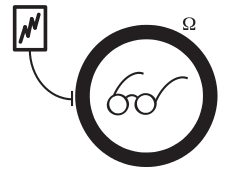
\includegraphics[width=0.25\textwidth]{1.png}
  \caption{Область $\Omega$, скрывающая объект от внешнего наблюдателя.}
  \label{fig:1}
\end{figure}

В общем случае, чтобы определить поведение электромагнитных полей, используют уравнения Максвелла, что необоснованно сложно для нашей задачи. Можно несколько упростить ее, если моделировать ситуацию при помощи волнового уравнения. Функция $u(x_1, x_2, t)$ удовлетворяет волновому уравнению, если $\frac{\partial^2 u}{\partial t^2} - c^2 \Delta u = 0$, где $c$ --- скорость света и $\Delta = \frac{\partial^2}{\partial x_1^2} + \frac{\partial^2}{\partial x_2^2}$ --- оператор Лапласа. Например, компоненты электрических и магнитных полей подчиняются волновому уравнению в пустом пространстве. Мы примем это упрощение на следующем шаге, рассматривая только стационарное или DC (direct current) отображение, в котором все величины не зависят от времени. Более того, внутренность области $\Omega$, даже когда там ничего не находится, будет состоять не из пустого пространства, а из электропроводящего материала. Как будет описано далее, наблюдатель использует измеренные электрические токи и напряжения чтобы представить себе, что находится внутри $\Omega$.


Давайте начнем с определения того, что мы подразумеваем, когда говорим, что внутренность $\Omega$ <<пуста>>. Материал называется однородным, если во всех точках его физические свойства одинаковы и изотропным, если его свойства не зависят от направления. Например деревянный брусок примерно однородный, но не изотропный, так как направление физические свойства зависят от направления волокон дерева. Материал, который не является изотропным называется анизотропным. Будем считать, что область $\Omega$ пуста, если она заполнена электропроводным однородным материалом, изотропным, в отношении электрической проводимости, это условие, при котором сторонний наблюдатель сможет найти $\Omega$. Конечно, если мы поместим внутрь $\Omega$ предмет, он не обязательно будет иметь такие же электрические свойства и изменит направление течения электрического тока внутри $\Omega$. Это изменение может быть использовано для обнаружения и отображения объекта извне.

\subsubsection{Изотропная проводимость}


Пусть $u(x_1, x_2)$ --- электрический потенциал (<<напряжение>>) в точке $(x_1, x_2) \in \Omega$. Электрическое поле $\textbf{E}$ (векторное поле) в $\Omega$ удовлетворяет $\textbf{E} = - \nabla u$. Электрическое поле толкает электроны порождает течение электрического тока, мы будем использовать обычную модель для этого явления, в которой позитивно заряженные потоки электронов игнорируются. Пусть $\textbf{J}$ определяет векторное поле тока в $\Omega$. Простейшая модель как $\textbf{J}$ зависит от $\textbf{E}$, а следовательно и от  $u$ --- это

\begin{equation}\label{Om}
\textbf{J} = \gamma \textbf{E}
\end{equation}

где $\gamma$ --- коэффициент \textit{проводимости}. В случае однородного изотропного материала $\gamma$ --- неотрицательная константа, в более общем случае $\gamma$ может быть функцией, зависящей от позиции $(x_1, x_2)$, или, в анизотропном случае, матрицей. Уравнение (\ref{Om}) в некотором смысле просто двумерная версия закона Ома, которая устанавливает линейную связь между электрическим полем и потоками тока, с током, всегда протекающим, в направлении  $\textbf{E}$. Если $\gamma$, то при заданном электрическом поле протекает много тока, в то время как при $\gamma$ близких к нулю тока фактически нет. Предельный случай, когда $\gamma = 0$ отвечает идеальному изолятору, не важно какой силы электрическое поле --- ток не идет.


Из $\textbf{E} = - \nabla u$ и (\ref{Om}) получаем:

\begin{equation}\label{dep}
\textbf{J} = -\gamma \nabla u.
\end{equation}
Если электрический заряд сохраняется в $\Omega$, как и должно быть, если внутри нет источника тока, получаем $\nabla \cdot \textbf{J} = 0$
всюду внутри $\Omega$. C \ref{dep} это означает

\begin{equation}\label{eq}
\nabla \cdot \gamma \nabla u = 0 \text{\;в\;} \Omega.
\end{equation}
В особом случае, когда $\gamma$ константа (то есть $\Omega$ пусто) мы можем упростить (\ref{eq}) до \textit{уравнения Лапласа}:

\begin{equation}\label{laplac}
\Delta u = 0 \text{\;в\;} \Omega,
\end{equation}
где $u = u(x_1, x_2)$. Это дифференциальное уравнение в частных производных, которому внутри однородного изотропного проводника должен удовлетворять электрический потенциал $u$. Функции, удовлетворяющие \ref{laplac} называются \textit{гармоническими}. Легко видеть, что любая постоянная функция $u$ удовлетворяет \ref{laplac} (что отвечает нулевому току всюду $\Omega$ \ref{dep}). Гораздо более интересный случай возникает, когда ток отличен от нуля, что требует неконстантный потенциал в $\Omega$.


Как можно получить отличный от константы потенциал в $\Omega$? Индуцируя неконстантный потенциал $f$ на $\partial \Omega$, например, прикрепить электроды к $\partial \Omega$ так, что
\begin{equation}\label{dirichle}
u = f \text{\;на\;} \partial \Omega,
\end{equation}
для некоторой выбранной функции $f$. Уравнение \ref{dirichle} --- граничное условие \textit{Дирихле}.


Уравнение Лапласа (\ref{laplac}) и граничное условие Дирихле (\ref{dirichle}) вместе образуют стандартную краевую задачу с единственным решением $u$ для некоторого приемлемого, например непрерывного, применяемого потенциала $f$. Но мы еще не учли наличие объекта в области, так как \ref{laplac} подходит только для пустого контейнера $\Omega$. Далее мы покажем, как моделировать и обнаруживать присутствие непроводящей <<дыры>> в $\Omega$.


\textit{Exercise 1.\;} Пусть мы параметризовали границу диска обычным образом: $x_1 = \cos \theta, x_2 = \sin \theta, 0 \le \theta \le 2 \pi$, а функция $f$  отвечающая условиям Дирихле на границе области в точке будет иметь вид $f(\theta) = a \cos \theta + b \sin \theta + c$ для любых констант $a, b ,c$. Покажите, что решением (\ref{laplac})-(\ref{dirichle}) будет гармоническая функция $u(x_1, x_2) = a x_1 + b x_2 + c$.

\subsubsection{Анизотропная проводимость}


Много материалов обладают анизотропными физическими свойствами. В контексте электропроводности это означает, что в любой заданной точке материал может в некоторых направлениях иметь лучшую проводимость, чем в других, и что принятая нами модель (\ref{Om}) с скалярной величиной $\gamma$ неприемлема. Можно обобщить (\ref{Om}), положив, что для любой взятой точки материал имеет направление наибольшей и наименьшей проводимости. Будем считать, что материал имеет максимальную проводимость $\gamma_M > 0$ в направлении единичного вектора $\textbf{v}_M$ и минимальную продуктивность $\gamma_m > 0$ в направлении единичного вектора $\textbf{v}_m$ так, что $0 < \gamma_m \le \gamma_M$. Так же естественно полагать, что векторы направлений $\textbf{v}_m$ и $\textbf{v}_M$ перпендикулярны друг другу. Модель, которая охватывает это поведение:

\begin{equation} \label{ani}
\textbf{J} = \sigma \textbf{E},
\end{equation}
где $\sigma$ --- симметричная, положительно определенная матрица $2 \times 2$, которая может зависеть от позиции, в силу симметричности и положительно определенности матрица имеет ортогональные собственные векторы и положительные собственные значения. Напомним, что матрица $\textbf{A}$ называется \textit{положительно определенной}, если  $\textbf{v}^{\textbf{T}}\textbf{Av} > 0, \forall \textbf{v} \ne 0$, $\textbf{v}^{\textbf{T}}$ --- транспонированный вектор $\textbf{v}$. Обратное так же верно: матрица с ортогональными собственными векторами и положительными собственными значениями является положительно определенной симметричной матрицей.


Для анизотропной проводимости (\ref{ani}) заменяет (\ref{dep}), и (\ref{eq}) становится

\begin{equation}
\nabla \cdot \sigma \nabla u = 0 \text{\;в\;} \Omega.
\end{equation}
Если электрическое поле $\textbf{E}$ применяется в направлении, параллельном $\textbf{v}_M$ тогда результирующий поток тока равен $\textbf{J} = \sigma \textbf{E} = \gamma_M \textbf{E}$ так, что $\| \textbf{J} \| = \gamma_M \| \textbf{E} \|$. Для фиксированных значений $\| \textbf{E} \|$ это направление для $\textbf{E}$ (параллельное $\textbf{v}_M$), максимизирует $\| \textbf{J} \|$. Смотри Упражнение 4 ниже. Аналогично, когда $\textbf{E}$ параллельно $\textbf{v}_m$ минимизирует $\| \textbf{J} \|$.


$\textit{Упражнение 2.\;}$ Какая матрица $\sigma\; 2 \times 2$ моделирует изотропный проводник с скалярной проводимостью $\gamma$ во всех направлениях?


$\textit{Упражнение 3.\;}$ Запишите матрицу анизотропной проводимости $\sigma$, моделирующую однородный материал с общей проводимостью $\gamma_M$ в направлении единичного вектора $\textbf{v}_M = \frac{\sqrt{2}}{2} i + \frac{\sqrt{2}}{2} j$ и проводимостью $\gamma_M$ в направлении единичного вектора $\textbf{v}_M = \frac{\sqrt{2}}{2} i - \frac{\sqrt{2}}{2} j$. \textit{Подсказка:}\; используйте факт, что $\sigma$ может быть представлена как $\sigma = \textbf{PD}\textbf{P}^{-1} = \textbf{PD}\textbf{P}^{-T}$, где $\textbf{P}$ --- матрица с собственными векторами матрицы $\sigma$ в качестве столбцов и $\textbf{D}$ --- диагональная матрица из собственных значений, в том же порядке, как столбцы $\textbf{P}$. Для заданной $\textbf{E}$, как ведет себя $\sigma \textbf{E}$ при $\gamma_m \to 0^{+}$?


$\textit{Упражнение 4.\;}$ Покажите, что если $\sigma$ --- симметричная, положительно определенная матрица $n \times n$ и мы зафиксируем $\| \textbf{v} \| = 1$, тогда $\| \sigma \textbf{v} \|$ максимально, когда $\textbf{v}$ --- собственный вектор для $\sigma$, отвечающий наибольшему(шим) собственному значению(ям). \textit{Подсказка:}\; мы можем записать

\begin{equation*}
\textbf{v} = \sum\limits_{k=1}^n \alpha_k \textbf{v}_k
\end{equation*}
где $\textbf{v}_k$ --- ортонормированные собственные вектора матрицы $\sigma$ и соответствующие им собственные значения упорядочены $0 < \lambda_1 \le \lambda_2 \le \dotsb \le \lambda_n$, тогда $\| \textbf{v} \|^2$ и $\| \sigma \textbf{v} \|^2$ могут быть выписаны явным образом через $\alpha_k$ и $\textbf{v}_k$.

\subsection{Импедансная томография}


В \textit{импедансной томографии} делается попытка изобразить внутреннюю часть $\Omega$ применяя электрический ток к $\partial \Omega$, скажем, прикрепляя несколько электродов к ней. Примененный ток индуцирует переменный в пространстве потенциал (то есть напряжение), через внутренность $\Omega$, который заставляет ток течь внутри области. Ток должен входить или покидать область через прикрепленные электроды, и результирующий потенциал на границе (который может быть измерен), зависит от внутренних свойств $\Omega$. Из этой информации: примененному току и результирующему потенциалу, можно восстановить информацию о внутренних электрических свойствах $\Omega$, таких как проводимость и тем самым формировать изображения. Смотри Рисунок \ref{fig:2} с примером изображений сердца и легких, полученных из реальной системы импедансного отображения. В статьях [5] и [11] можно найти хороший общий обзор этой темы.
\begin{figure}[t]
  \centering
  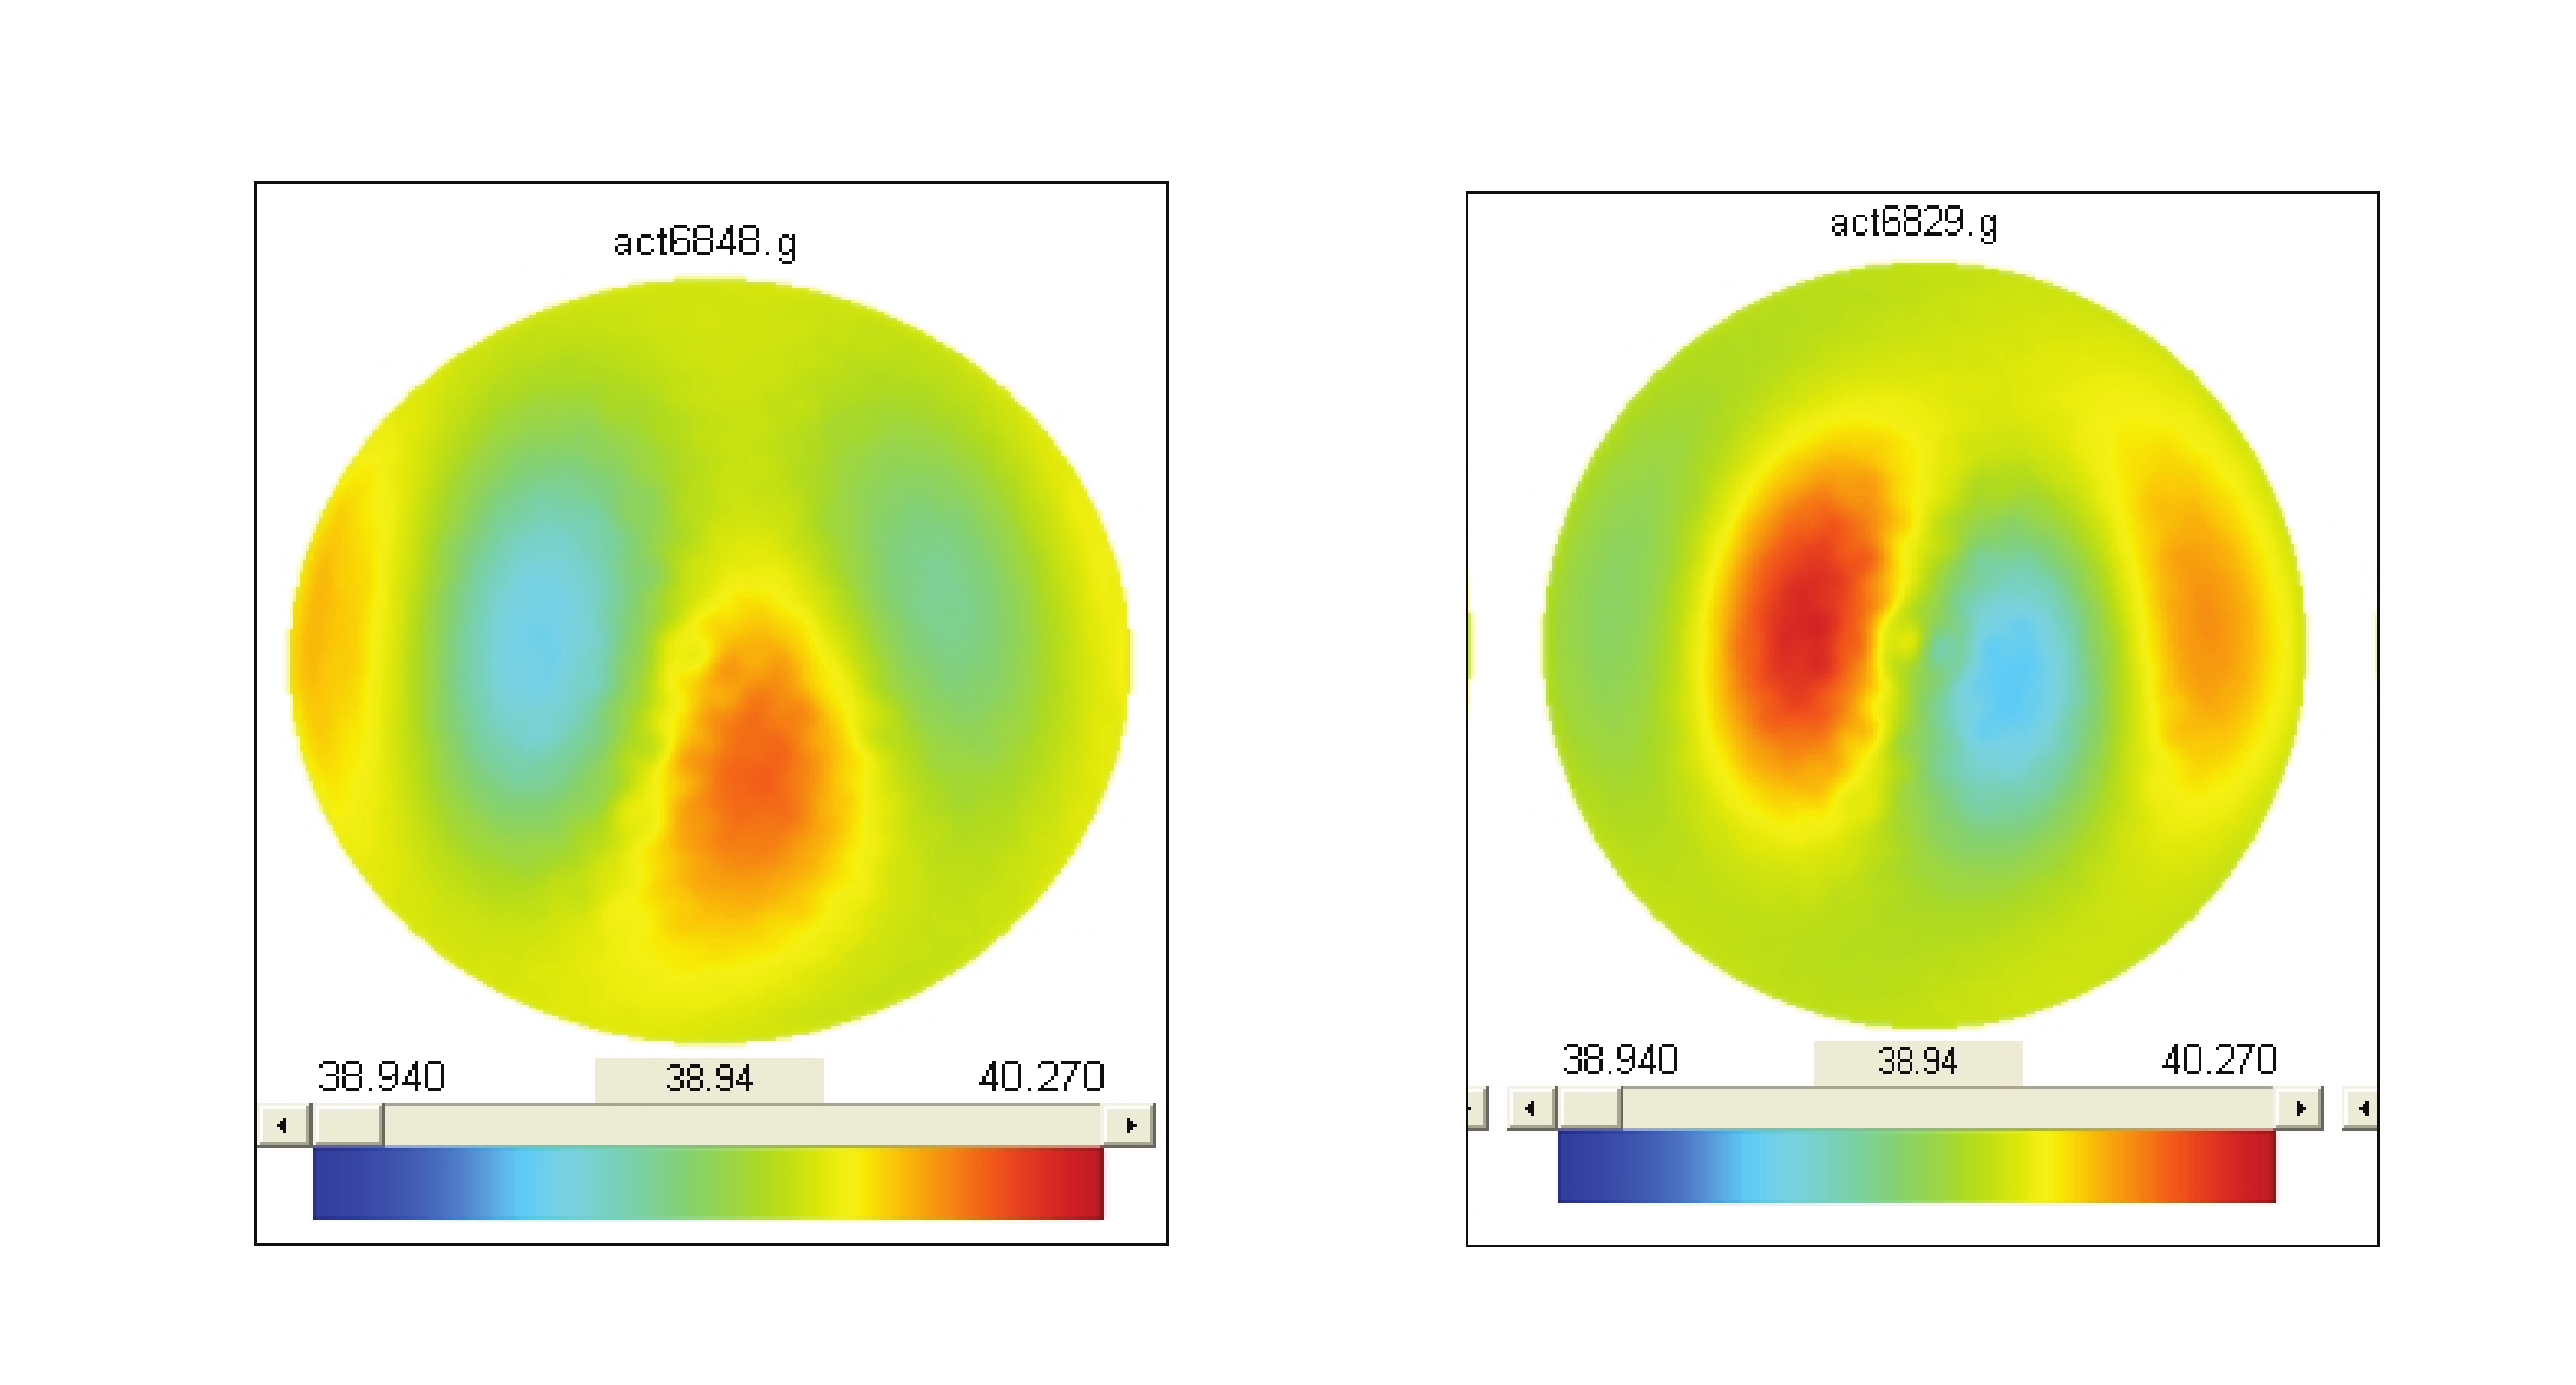
\includegraphics[width=0.5\textwidth]{2.png}
  \caption{Слева изображено импедансное отображение поперечного сечения туловища, когда кровь заполняла сердца и выходила из легких объекта.
  Область рядом с сердцем отмечена красным, так как проводимость в этот момент высока (кровь очень проводима). В противоположность, легкие, в которых в данный момент немного крови, окрашены в голубой. Справа кровь вышла из сердца и перешла в легкие, изменив цвета на противоположные}
  \label{fig:2}
\end{figure}

\subsubsection{Отображение пустот}


Давайте посмотрим, как можно с помощью этого подхода изображать определенный специальный тип объектов в $\Omega$. Мы используем эквивалентный, но математически более удобный способ применения потенциалов, а затем измерения текущего тока на границе $\partial \Omega$. Ключевым моментом является определение отображения между примененным потенциалом и результирующим током на границе и как это отображение зависит от внутренних свойств $\Omega$.


Для начала, будем считать $\Omega$ пустой, тогда имеем однородную изотропную проводимость $\gamma > 0$. Пусть внутрь $\Omega$ помещен непроводящий объект $D$, можно думать, что $D$ есть пустота, как пропавший материал. Когда на границу области применен потенциал $f$, имеющаяся там пустота должна изменять течение тока внутри $\Omega$, и этот эффект должен быть обнаруживаемым с границы.
Исследуемая нами величина --- это скорость, с которой электрический ток втекает в $\Omega$ в каждой точке $\partial \Omega$. Скорость, с которой ток вытекает рядом с точкой $p \in \partial \Omega = \textbf{J}(p) \cdot \textbf{n}(p)$, где $\textbf{n}(p)$ --- внешний единичный вектор нормали к $\partial \Omega$ в точке $p$. В дальнейшем будем пренебрегать зависимостью величин, таких как $\nabla u$ и $\textbf{n}$, от $p$. Применение (\ref{dep}) показывает, что ток, текущий по всей $\partial \Omega$ в любой точке равен $- \gamma \nabla u \cdot \textbf{n}$. Таким образом скорость, с которой ток \textit{входит} в $\partial \Omega$ есть $\gamma \nabla u \cdot \textbf{n}$ и называется $\textit{данные Неймана}$ для функции $u$.


Наличие $D$ в $\Omega$ меняет поток тока, и никакой ток не может проходить в $D$ из $\Omega \setminus D$. Это означает, что $\textbf{J} \cdot \textbf{n} = 0$ в $\partial D$, здесь $\textbf{n}$ обозначает единичный вектор нормали к $\partial D$, указывающий внутрь $D$ (из $\Omega \setminus D$). Из уравнения (\ref{dep}) вытекает $\gamma \nabla u = 0$ на $\partial \Omega$. В этом случае потенциал $u$ опеределен только в $\Omega \setminus D$ и подчиняется уравнению Лапласа, наряду с условием Дирихле (\ref{dirichle}) на $\partial \Omega$ и дополнительному граничному условию

\begin{equation}\label{dD}
\gamma \nabla u = 0 \text{\;на\;} \partial \Omega.
\end{equation}
Поскольку $\gamma > 0$ мы можем переписать (\ref{dD}) как $\frac{\partial u}{\partial t} = 0$, используя сокращенную запись для нормальной производной $\frac{\partial u}{\partial t} := \nabla u \cdot \textbf{n}$.


\textit{Пример 2.1} Пусть наблюдатель применяет потенциал $f(\theta) = \cos \theta + \sin \theta$ к границе диска. Из Упражнения 1, результирующий потенциал внутри диска будет $u(x_1, x_2) = x_1 + x_2$. Но если мы уберем(почему уберем, мы же его как раз добавили?) шар $D = B_{1/2}(\textbf{0})$, (здесь через $B_{r}(p)$ стандартно обозначен шар радиуса $r$ с центром в точке $p$, $\textbf{0} = (0, 0)$) тогда $u(x_1, x_2) = x_1 + x_2$ больше не будет потенциалом, наведенным в круговом кольце $\Omega \setminus D$ потенциалом $f$, так как $u$ не удовлетворяет (\ref{dD}). Чтобы это увидеть отметим, что $\partial D$ может быть параметризован как $x_1 = \frac{1}{2} \cos (\theta), x_2 = \frac{1}{2} \sin (\theta), n = -\cos (\theta) i - \sin (\theta) j$. Тогда

\begin{equation*}
\nabla u \cdot \textbf{n} = (i + j) \cdot (-\cos (\theta) i - \sin (\theta) j) = -(\cos(\theta)+\sin(\theta)),
\end{equation*}
что не совсем равно нулю на $\partial D$. Действительно, в этом случае
правильный потенциал внутри $\Omega \setminus D$ равен $u(x_1, x_2) =
(x_1 + x_2)(4x_1^2 + 4x_2^2 + 1)/(5x_1^2 + 5x_2^2)$. Смотри Рисунок
\ref{fig:3} с графиками потока тока в каждом случае. Непроводящая
пустота мешает протеканию тока, наблюдатель измеряет, в полярных
координатах $(r, \theta)$, $\frac{\partial u}{\partial \textbf{n}}(1,
\theta) = \frac{3}{5}(\cos(\theta)+\sin(\theta))$ на $\partial
\Omega$, сравнивая с $\frac{\partial u}{\partial \textbf{n}}(1,
\theta) = \cos(\theta)+\sin(\theta)$ для цельного единичного диска.
\begin{figure}[t]
  \centering
  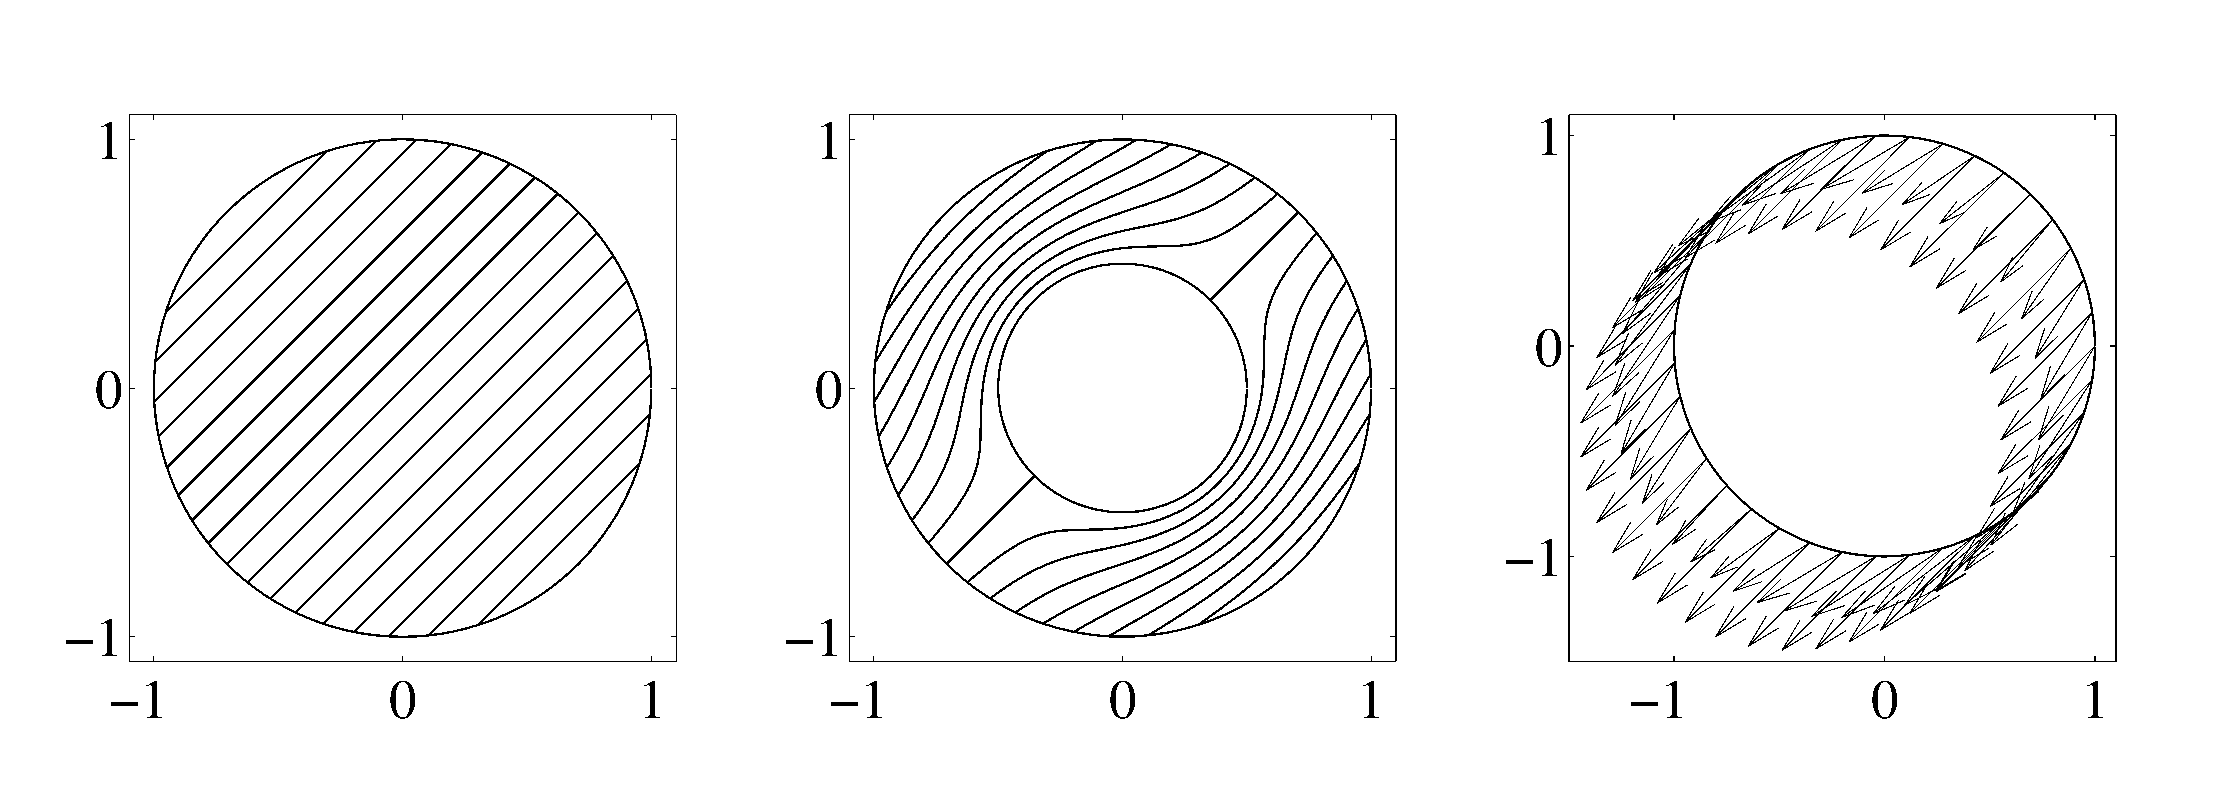
\includegraphics[width=0.5\textwidth]{3.png}
  \caption{Сравнение решений в единичном диске и кольце. Первый график показывает течение линий тока
    $\mathbf J = -\gamma \nabla u$, где $u$ --- решение уравнения Лапласа в граничными условиями Дирихле $f(\theta) =
    cos(\theta) + sin(\theta)$ (потенциал, примененный наблюдателем) на внешнюю границу единичного диска. Поток, показанный на среднем графике имеет тот же самый примененный потенциал  $f$ на внешней границе, плюс условие Неймана нулевого потока на внутренней границе диска
    $1/2 \leq r \leq 1$. На третьем графике сравнивается $\mathbf J$ на границе диска и кольца, где более короткие стрелки отвечают  $\mathbf J$ для кольца.}
  \label{fig:3}
\end{figure}


\textit{Упражнение 5.\;} Убедитесь, что функция $u(x_1, x_2) = (x_1 + x_2)(4x_1^2 + 4x_2^2 + 1)/(5x_1^2 + 5x_2^2)$ из Примера 2.1 является гармонической функцией на $\Omega \setminus D$, где $D = B_{1/2}(\textbf{0})$, с $u = \cos(\theta)+\sin(\theta)$ на $\partial \Omega$ и $\nabla u \cdot \textbf{n} = 0$ на $\partial D$.
\subsubsection{Обратные задачи и Маскировка}


Все вышесказанное предлагает вариант процедуры импедансной визуализации для сбора информации о внутренности $\Omega$, в этом случае, найдя в области дыру:
\begin{enumerate}
  \item Применить потенциал $f$ к границе области (уравнение (\ref{dirichle}))
  \item Измерить ответ $\gamma \nabla u \cdot \textbf{n}$ на $\partial \Omega$ (результирующий ток).
\end{enumerate}
Из такого типа <<стимулов-ответов>> или данных Дирихле-Неймана мы хотим определить точный размер, форму и положение дыры $D$. Конечно, шаги 1 и 2 можно повторять с различными входными потенциалами $f$, которые могли бы дать дополнительную информацию. Импедансная визуализация это пример обратной задачи. Определение обратной задачи не высечено на камне, но грубо может быть дано как <<выяснение причин из следствий>>. В контексте дифференциальных уравнений это принимает вид выяснения коэффициентов уравнения из знания о решениях, в противовес прямой задаче нахождения решения определенного дифференциального уравнения с заданными коэффициентами. В нашем случае обратная задача состоит в определении какой внутренний регион $D$ мог вызвать измеренный на границе ток для примененного потенциала $f$, вместо того, чтобы по заданным $f$ и $D$ посчитать ток на границе путем решения дифференциального уравнения. Обратные задачи такого типа часто возникают в приложениях, где требуется определить внутреннею структуру из внешних измерений.


У нас под рукой есть зачатки сырой маскировки. Если мы хотим спрятать проводящий объект внутри $\Omega$, всего лишь требуется выкопать непроводящее отверстие некоторого радиуса $\rho > 0$ и поместить объект внутри. Таким образом, объект изолирован от внешнего мира и не может быть увиден с помощью импедансного отображения. К сожалению, само отверстие может быть обнаружено, так что наблюдатель будет знать, что внутри что-то спрятано, даже если он и не узнает что это. С таким же эффектом Гарри Поттер заменил бы свою мантию невидимку на простынь.


Тем не менее, идея выкапывания ямы в которую можно положить что-нибудь это начало жизнеспособной маскировки, но сначала, нам нужно проанализировать уравнение Лапласа в кольце $\Omega \setminus B_{\rho}(\textbf{0})$ более тщательно.

\subsection{Решение уравнения Лапласа в кольце}
Пусть $D = B_{\rho}(\textbf{0})$, так же, как посередине Рисунка \ref{fig:3} с $\rho < 1$. Наша цель определить $\rho$ используя импедансное отображение. Простой способ сделать это --- решить уравнение Лапласа с граничными условиями (\ref{dirichle})-(\ref{dD}) в явном виде, чтобы увидеть, что значение $\rho$ на самом деле содержится в данных Неймана $\gamma \nabla u \cdot \textbf{n}$ на $\partial \Omega$. Решение уравнения Лапласа может быть получено стандартным разделением переменных в полярных координатах, что будет и сделано далее. Больше информации о методе разделения переменных для решения дифференциальных уравнений смотри [27].


В дальнейшем, просто для удобства, будем считать $\gamma = 1$.


Область $\Omega \setminus D$ --- кольцо, значит удобно записать уравнение Лапласа (\ref{laplac}) в полярных координатах
\begin{equation}\label{polar}
\frac{\partial^2 u}{\partial r^2} + \frac{1}{r} \frac{\partial u}{\partial r} + \frac{1}{r^2} \frac{\partial^2 u}{\partial \theta^2} = 0,
\end{equation}
где $u = u(r, \theta)$ это потенциал в $\Omega \setminus D$. Используя (\ref{polar}), легко видеть, что функции $1, \ln(r)$ и $r^{|k|} e^{ik\theta}, r^{-|k|}e^{ik\theta}$ грамоничны, для всех $k \in \mathbb{Z}, r > 0$ и, следовательно, на кольце $\Omega \setminus D$. Мы построим необходимое решение $u(r, \theta)$ как суперпозицию этих функций,

\begin{equation}\label{sol}
u(r, \theta) = c_0 + d_0\ln(r) + \sum\limits_{k \in \mathbb{Z} \setminus \{0\}}{(c_k r^{|k|} + d_k r^{-|k|}) e^{ik\theta}},
\end{equation}
правильно подбирая коэффициенты $c_k, d_k$.


Граничное условие Дирихле $u = f$ на $\partial \Omega$ означает $u(1, \theta) = f(\theta)$, тоесть

\begin{equation}\label{fd}
c_0 + \sum_{k \in \mathbb{Z} \setminus \{0\}}{(c_k + d_k)e^{ik\theta}} = f(\theta), \theta \in [0, 2\pi).
\end{equation}
(\ref{fd}) выглядит как ряд Фурье для $f$. Мы предполагаем, что $f$ ведет себя достаточно хорошо, например, непрерывна и кусочно дифференцируема, следовательно ряд Фурье поточечно сходится к $f$. Можно разложить $f$ в ряд Фурье как

\begin{equation*}
f(\theta) = \sum_{k \in \mathbb{Z}}{f_k e^{ik\theta}}, \text{\;где\;} f_k = \frac{1}{2 \pi} \int^{2 \pi}_{0}{f(\theta)e^{-ik\theta} d\theta}.
\end{equation*}
Сопоставляя $f_k$ с соответствующими слагаемыми слева в (\ref{fd}) заключаем

\begin{equation}
c_0 = f_0 \text{\;и\;} c_k + d_k = f_k \forall k \in \mathbb{Z} \setminus \{0\}.
\end{equation}


Чтобы завершить вычисления воспользуемся граничным условием Неймана \ref{dD}, которое принимает вид $\frac{\partial u}{\partial r} = 0$ на $\partial D$ (используя тот факт, что векторное поле $\mathbf{n}$ на $\partial D$ указывает в радиальном направлении к началу координат так, что $\frac{\partial}{\partial \mathbf{n}} = -\frac{\partial}{\partial r}$ вдоль этой внутренней границы). Формально почленно дифференцируя \ref{sol} по $r$, а затем вычисляя в точке $r=\rho$ приводит к

\begin{equation}\label{e13}
\frac{d_0}{\rho} + \sum_{k \in \mathbb{Z} \setminus \{0\}}{|k|(c_k \rho^{|k|-1} - d_k \rho^{-|k|-1})e^{ik\theta}} = 0 \forall \theta \in [0, 2 \pi).
\end{equation}
Выражение (\ref{e13}) может быть интерпретировано как ряд Фурье для нулевой функции, чьи коэффициенты Фурье равны нулю, поэтому можно записать

\begin{equation}
d_0 = 0,
\end{equation}
\end{document}
